\documentclass{article}
\usepackage{../verslagstyle}



\begin{document}
	\title{Labo 3}
	\author{Bert De Saffel}
	\date{26 februari 2019}
	\maketitle
	
	\section{Oplosmethode}
	Aangezien het eindresultaat geen gaten vertoond in de verticale richting is dit een geval van closure, maar enkel voor de y-richting. Er wordt eerst dilatatie uitgevoerd in de y-richting, zodat de vorm van de bollen in elke kolom verdwijnt, en dat het de vorm van een rechthoek krijgt met een bepaald kleurenspectrum. Daarna wordt erosie uitgevoerd om deze rechthoeken te versmallen in de x-richting.
	
	\section{Gebruikte functies}
	\begin{itemize}
		 \item \textbf{getStructuringElement(shape, ksize[, anchor]) $\rightarrow$ retval}
		 
		 Deze functie geeft een matrix terug die typisch kan gebruikt worden voor morfologische operaties. In dit labo worden er twee matrices $D$ en $E$, die respectievelijk gebruikt worden bij het dilatatie- en erosieproces, gedefinieerd:
		 
		 
		 $$D = \begin{pmatrix}
		  1 \\ 1 \\ 1 \\ 1 \\ 1
		 \end{pmatrix} \qquad 
		 E = \begin{pmatrix}
		 1 & 1 & 1 \\
		 1 & 1 & 1 \\
		 1 & 1 & 1
		 \end{pmatrix}
		 $$
		 
		 
		Om deze matrices te genereren is de waarde \textit{shape} gelijk aan \texttt{cv2.MORPH\_RECT} en de waarde van \textit{ksize} gelijk aan \texttt{(1, 5)} voor matrix $D$ en \texttt{(3, 3)} voor matrix $E$.
		 
		 \item \textbf{dilate(src, kernel[, ..., iterations, ...]) $\rightarrow$ dst}
		 
		 Deze functie zal dilatatie uitvoeren op de gegeven \textit{src} gebruik makend van de gegeven \textit{kernel}. De \textit{iterations} parameter geeft het aantal keer aan dat dilatatie zal uitgevoerd worden. Aangezien matrix $D$ slechts 1 kolom heeft, wordt er enkel rekening gehouden met pixels direct boven of direct onder de pixel in het centrum waar de kernel zich op dat moment bevindt, zodat de bollen enkel uitgesmeerd worden over de y-as. Het is noodzakelijk dat er nog zwarte pixels bestaan tussen twee opeenvolgende kolommen, anders kan het erosieproces nooit deze zwarte pixels opnieuw genereren. De gekozen matrix $D$ met drie iteraties levert de beste resultaten op, zoals te zien op figuur \ref{Fig:ex2_2}.
		 
		 \item \textbf{erode(src, kernel[, ..., iterations, ... ]) $\rightarrow$ dst}
		 
		 Deze functie heeft dezelfde parameters als \textit{dilate}, maar zal dan erosie uitvoeren. Na de dilatatie stap zijn de bollen uitgesmeerd zodat elke kolom nu een rechthoek is. Deze rechthoeken kunnen in de x-richting versmalt worden door erosie toe te passen. Door erosie drie maal toe te passen met matrix $E$ wordt het resultaat zoals op figuur \ref{Fig:ex2_3} bekomen. De dimensies van de matrix zijn vrij te kiezen, zolang dat het aantal iteraties ook maar aangepast wordt. Een 4X4 matrix met slechts 2 iteraties of een 2X2 matrix met 5 iteraties leveren nagenoeg dezelfde resultaten op. Een te grote matrix kan met 1 iteratie wel al te veel verdunnen. Het beste is om empirisch na te gaan wat de beste combinatie van matrixgrootte en aantal iteraties is.
		 

		 
		
		
	\end{itemize}
	\section{Invoer en uitvoer}

	\subsection*{Opgave 7}
	\begin{figure}[!htb]
		\begin{minipage}{0.3\textwidth}
			\centering
			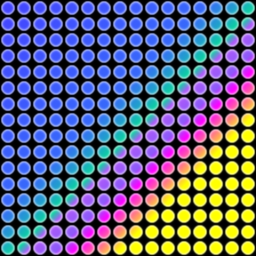
\includegraphics[width=0.9\linewidth]{rainbowdiscs}
			\caption{De originele figuur.}
			\label{Fig:ex2_1}
		\end{minipage}\hfill
		\begin{minipage}{0.3\textwidth}
			\centering
			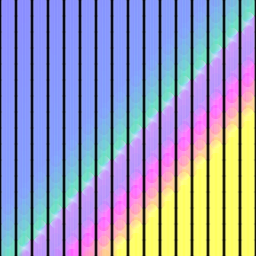
\includegraphics[width=0.9\linewidth]{rainbowdiscsEX7DILATATION}
			\caption{Na de dilatatie.}
			\label{Fig:ex2_2}
		\end{minipage}\hfill
		\begin{minipage}{0.3\textwidth}
			\centering
			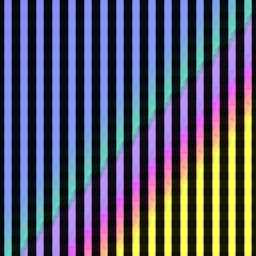
\includegraphics[width=0.9\linewidth]{rainbowdiscsEX7EROSION}
			\caption{De erosie na de dilatatie.}
			\label{Fig:ex2_3}
		\end{minipage}
	\end{figure}

	
\end{document}